%% 明石研究室修士論文テンプレート

\documentclass[a4paper,12pt,titlepage]{jarticle}
\usepackage[dvipdfmx]{graphicx}
\usepackage{color}
\usepackage{amsmath,amssymb,bm}
\usepackage{wrapfig}
\usepackage{url}
\usepackage{afterpage}
\usepackage{ascmac}
\usepackage{array}
\usepackage{geometry}
\usepackage{emathC}
\usepackage{itembkbx}
\usepackage{itembbox}
\usepackage{eclbkbox}
\usepackage{here}
\usepackage{listings, jlisting}
\usepackage{comment}

\renewcommand{\lstlistingname}{リスト}
\lstset{language=c,
  basicstyle=\ttfamily\scriptsize,
  commentstyle=\textit,
  classoffset=1,
  keywordstyle=\bfseries,
  frame=tRBl,
  framesep=5pt,
  showstringspaces=false,
  numbers=left,
  stepnumber=1,
  numberstyle=\tiny,
  tabsize=2
}
\geometry{top=2.5cm,bottom=2.5cm,left=3.1cm,right=3.1cm}
  \makeatletter
  \newcommand{\subsubsubsection}{\@startsection{paragraph}{4}{\z@}%
    {1.0\Cvs \@plus.5\Cdp \@minus.2\Cdp}%
    {.1\Cvs \@plus.3\Cdp}%
    {\reset@font\sffamily\normalsize}
  }
  \makeatother
  \setcounter{secnumdepth}{4}



% 表紙情報
\title{
{\Large 平成27年度 東京理科大学大学院 修士論文 \\[3cm]}
{\Huge レーザー光を用いた\\ハンドジェスチャーの\\拡張現実への応用 \\[3cm]}
{\Large 東京理科大学大学院 理工学研究科 情報科学専攻 \\
明石研究室 修士課程2年\\[2cm]}
}
\author{学籍番号 6313640 \\
渡部 祐太}
\date{}



\begin{document}
% 表紙
\maketitle
% 目次
\tableofcontents



% 本文
\newpage
% 1
\section{序論}

% 1.1
\subsection{背景}
我々は、PCを操作する際にマウス、キーボードを使用する。しかしながら、これらのインターフェースを使いこなすのには時間が必要であり、直感的に扱えるインターフェースとは決して言うことはできない。この問題を解決する一例として、ハンドジェスチャーが挙げられる。この技術により、簡単な操作であれば直感的に行うことができるようになり、より多くの人々が扱うことができる。その一方で、ジェスチャーの種類には限りがあるため、操作が複雑になればなるほど、それを純粋なジェスチャーのみで表現することは難しくなってしまう。そこで、近年ではVR技術と組み合わせることにより、この欠点を補う試みが多々見られる。これにより、多くのシチュエーションに対して、ジェスチャーによる操作を応用することが可能になるため、今後、ハンドジェスチャーはより生活に密接した存在になることが予想される。だが、この進歩の途上には一つの新しい問題が存在する。それは、カメラ等の既存のセンサーが使用できない場所での、ジェスチャーの使用が求められる、というものである。具体例を挙げると、トイレのような倫理的にカメラの使用が憚られる場所がある。この場所では、非接触型インターフェースとして、ハンドジェスチャーの需要が高まると予想されるにも関わらず、カメラをセンサーとして使用した既存の技術は使用することができない。そのような状況への対策として、カメラ以外のセンサーを用いたハンドジェスチャー技術が求められている。

% 1.2
\subsection{目的}
主に二つのことを主眼を置いている。一つ目は、ハンドジェスチャーとVR技術を組み合わせることによって、直感的な操作を行うことができるインターフェースの提案をする。二つ目は、ジェスチャーを認識するセンサーとして、カメラを使用しないことにより、これまで利用できなかったシチュエーションでもジェスチャーを利用可能にする、ということである。

% 1.3
\subsection{構成}
本論文は、全六章から構成される。第二章では、本論文において必要となる技術や用語等を紹介する。第三章では、研究の概要と提案手法を記述する。第四章では、提案したシステムの具体的なアルゴリズムを説明する。第五章では、アルゴリズムを実際にどのように実装したのかを、プログラムを交えつつ説明する。第六章では、システムを動作させた結果を提示する。最後に、第七章では、これらのことを踏まえて、考察、結論等の総括を行う。	% 序論
\newpage
% 2
\section{関連用語}

% 2.1
\subsection{VR}
VR についての説明

% 2.2
\subsection{Unity}
Unity についての説明

% 2.3
\subsection{OpenCV}
OpenCV についての説明	% 類似研究
\newpage
% 3
\section{研究概要}

% 3.1
\subsection{概要}
ハンドジェスチャーを使用する際に用いられるセンサーとして、一般的とされているWebカメラではなく、レーザー光を用いる。このことは、従来ジェスチャーを使用できなかったシチュエーションや場所においても、使用することを可能とする。

具体的なレーザー光の使用方法を説明する。多数のレーザーと、それと同数の受光器を用意して、お互いが対面するように配置することにより、その間を手が遮った際に検出できるようにする。この検出した情報から手のおおよその形状を認識する。予め3Dオブジェクトを配置した、3Dの仮想空間を用意して、そこに取得した手の形状を描画し、3Dオブジェクトを動かすことができるようにする。このことで、レーザー光を用いたデバイスがインターフェースとして使用することができることを証明する。

本研究では、これを2台のWebカメラを用いて作ったシミュレータデバイスを用意して実験を行う。

% 3.2
\subsection{提案手法}
\subsubsection{レーザー光デバイス}
レーザー光を用いたハンドジェスチャーを可能とするため、図1のようなデバイスを作成した。

デバイスの上部に、計24個のレーザーを設置する。それと対になるように、下部に同数の受光器を設置する。この間を手が通過すると、レーザー光が遮られたことを受光器が検出する。実際に作成したデバイスを用いて、取得した手情報を画像に描画したものを、図2に示す。図3は使用したデバイスの写真である。

図2より、レーザー光を用いて手の形状を認識することが可能であることが伺える。しかしながら、このデバイスには問題が存在する。それは、レーザー数が足りないため、手の情報を得るためには、スキャナーのように手を固定した形で通過させる必要がある。このことは動的な手情報を得ることができないことを示している。つまり、VRと組み合わせた直感的なハンドジェスチャーインターフェースを作ることは、不可能である。だが、図2の結果から、手の範囲より広くレーザーを設置することが出来れば、動的に手情報を得ることができると推測される。% このデバイスのイメージ用意してもいいかも
このことを踏まえて、レーザー光の代わりにWebカメラを用いたシミュレータデバイスを作成した。

\subsubsection{Webカメラを用いたシミュレータデバイス}	% 研究概要
\newpage
% 4
\section{研究概要}



% 4.1
\subsection{概要}
ハンドジェスチャーを使用する際に用いられるセンサーとして、一般的とされているWebカメラではなく、レーザー光を用いる。このことは、従来ジェスチャーを使用できなかったシチュエーションや場所においても、使用することを可能とする。

具体的なレーザー光の使用方法を説明する。多数のレーザーと、それと同数の受光器を用意して、お互いが対面するように配置することにより、その間を手が遮った際に検出できるようにする。この検出した情報から手のおおよその形状を認識する。予め3Dオブジェクトを配置した、三次元の仮想空間を用意して、そこに取得した手の形状を描画し、3Dオブジェクトを動かすことができるようにする。このことで、レーザー光を用いたデバイスがインターフェースとして使用することができることを証明する。

本研究では、これを2台のWebカメラを用いて作ったシミュレータデバイスを用意して実験を行う。



% 4.2
\subsection{提案手法}
\subsubsection{レーザー光デバイス}
レーザー光を用いたハンドジェスチャーを可能とするため、図3-1のようなデバイスを作成した。

\begin{center}
  \includegraphics[width=10cm]{RazerDevice_image} \\

 \vspace{1mm}
  図3-1. レーザー光を用いたデバイスのイメージ
\end{center}

デバイスの上部に、計24個のレーザーを設置する。それと対になるように、下部に同数の受光器を設置する。この間を手が通過すると、レーザー光が遮られたことを受光器が検出する。実際に作成したデバイスを用いて、取得した手情報を画像に描画したものを、図3-2に示す。図3-3は使用したデバイスの写真である。

\begin{center}
  \includegraphics[width=10cm]{RazerDevice_getInfo.eps} \\

 \vspace{1mm}
  図3-2. レーザー光デバイスを用いて実際に得た情報
\end{center}

 \vspace{5mm}

\begin{center}
  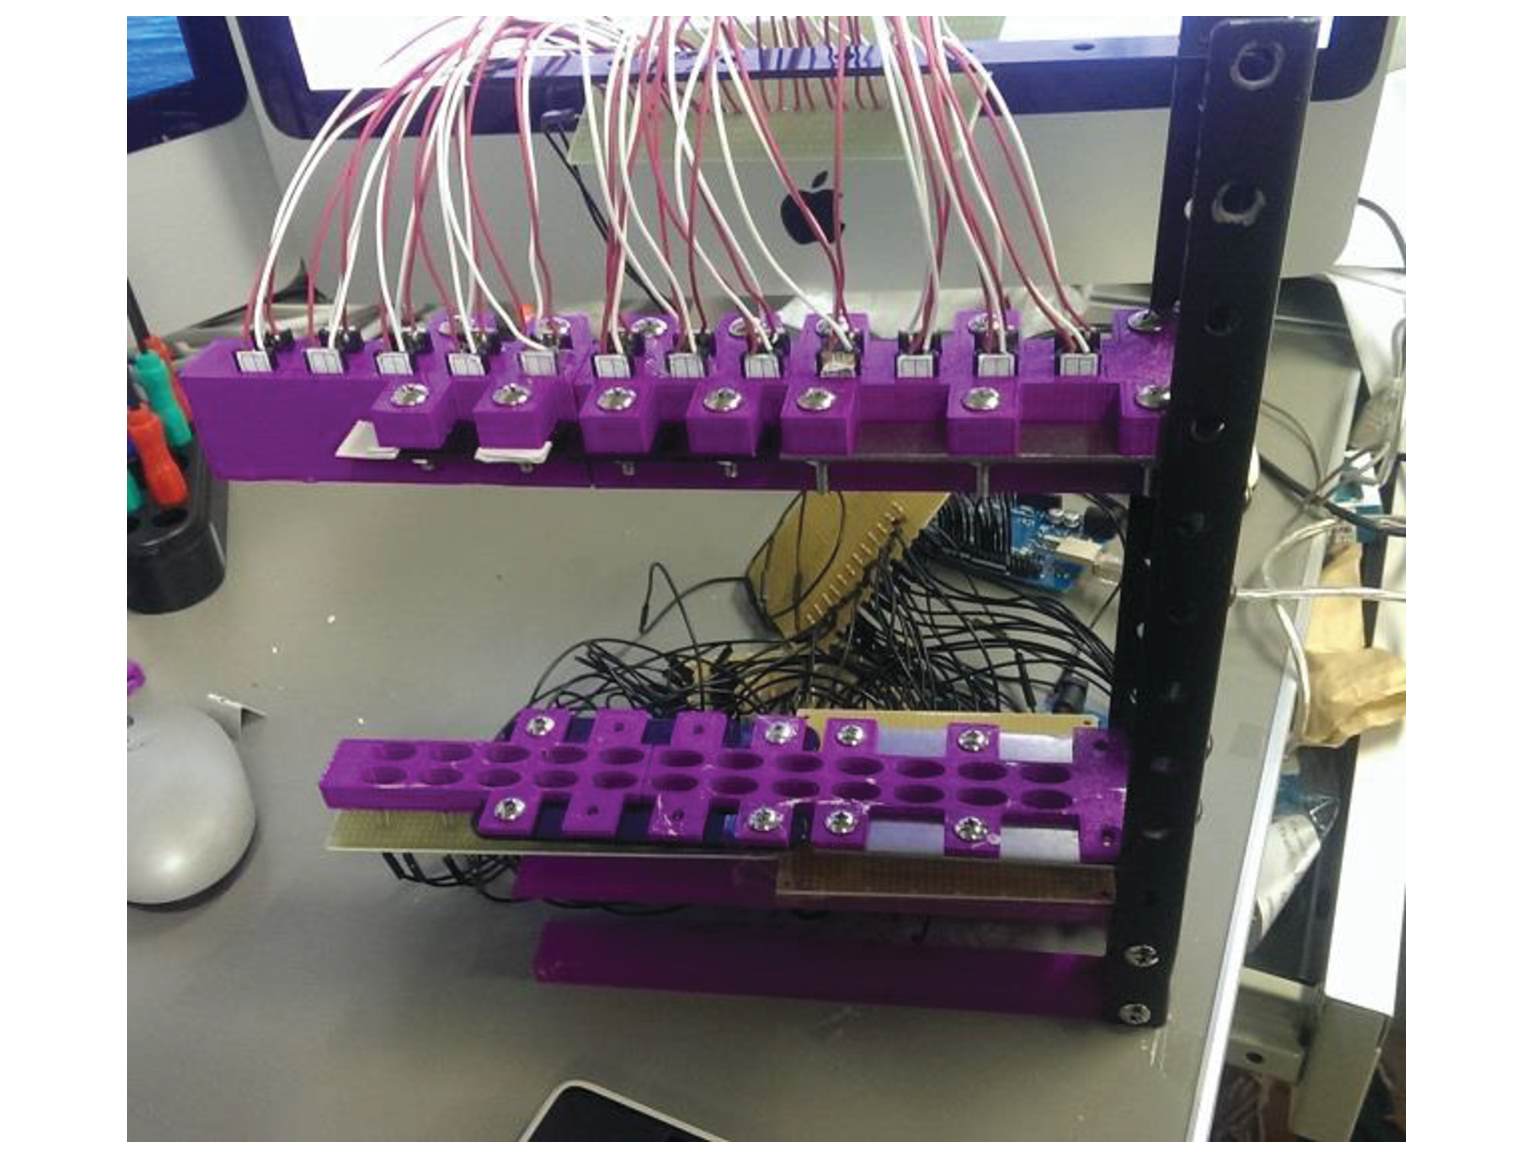
\includegraphics[width=10cm]{RazerDevice_real_color.eps} \\

 \vspace{1mm}
  図3-3. 実際に作成したレーザー光デバイス
\end{center}

図3-2より、レーザー光を用いて手の形状を認識することが可能であることが伺える。しかしながら、このデバイスには問題が存在する。それは、レーザー数が足りないということである。手の情報を得るためには、スキャナーのように手を固定した形で通過させる必要がある。このことは動的な手情報を得ることができないことを示している。つまり、VRと組み合わせた直感的なハンドジェスチャーインターフェースを作ることは、不可能である。だが、図3-2の結果から、手の範囲より広くレーザーを設置することが出来れば、動的に手情報を得ることができると推測される。% このデバイスのイメージ用意してもいいかも
このことを踏まえて、レーザー光の代わりにWebカメラを用いたシミュレータデバイスを作成した。

\subsubsection{Webカメラを用いたシミュレータデバイス}
図3-4は、レーザー光の代わりにWebカメラを用いたシミュレータデバイスのイメージとなる。側面が一つ空いているボックスの上面と側面に対して、図3-4のようにWebカメラを設置する。レーザー光による検出を再現するために、Webカメラから得られた映像に対して、一定間隔毎に情報を取得する座標を設ける。カメラの対面には、青いスクリーンを貼り付けることにより、間を青以外の物体が遮った時、それを検出できるようにする。実際にボックスの中に手を入れて、取得した情報を図3-5に示す。図3-5は図3-4の上部に設置したWebカメラから取得した情報である。同様の手法で、横のWebカメラからも同時に情報を取得する。縦、横の二つの画像から手情報を三次元空間に構築して、同空間に生成したオブジェクトを動かすことにより、直感的なジェスチャーを可能にするための道筋を示す。図3-6は実際に作成したシミュレータデバイスである。

\begin{center}
  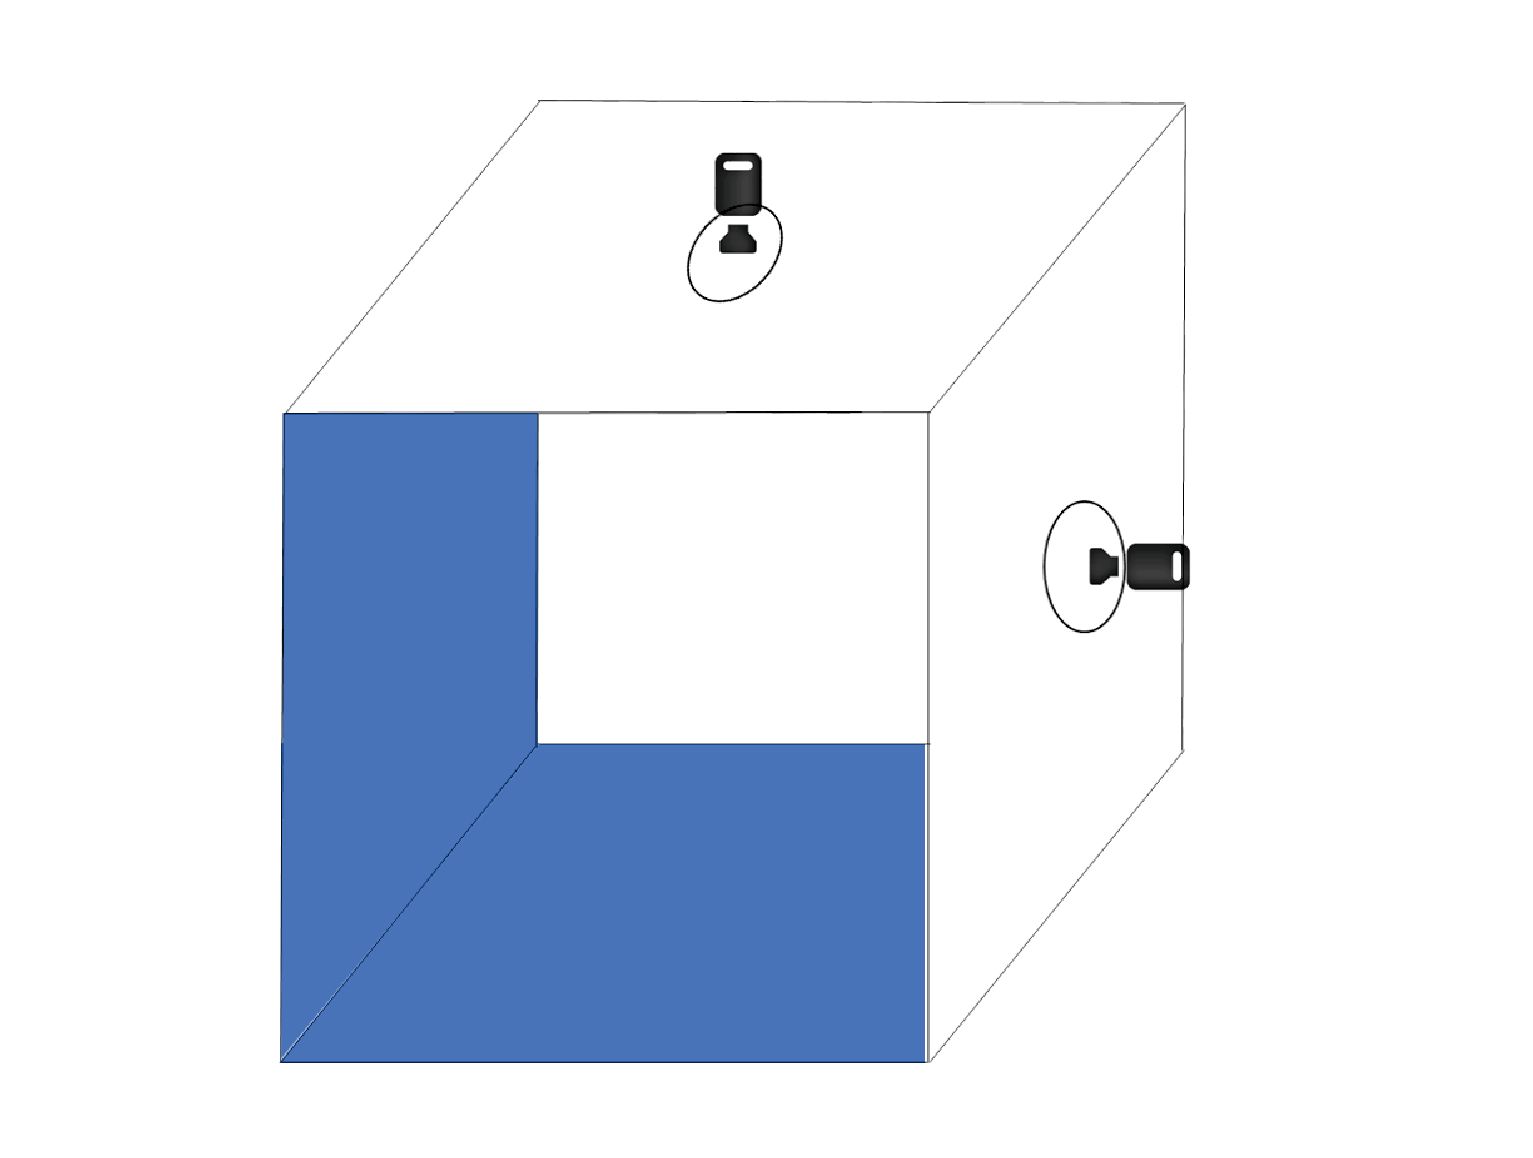
\includegraphics[width=10cm]{Simulator_image.eps} \\

 \vspace{1mm}
  図3-4. Webカメラを用いたシミュレータデバイスのイメージ
\end{center}

\begin{center}
  \includegraphics[width=10cm]{Simulator_getInfo.eps} \\

 \vspace{1mm}
  図3-5. シミュレータデバイスから得られた情報
\end{center}

 \vspace{10mm}
\begin{center}
  \includegraphics[width=10cm]{Simulator_real_color.eps} \\

 \vspace{1mm}
  図3-5. 実際に作成したシミュレータデバイス
\end{center}	% アルゴリズム
%\newpage
%% 6
\section{実験}

% 6.1
\subsection{環境}
環境を記述

% 6.2
\subsection{結果}
結果を記述	% 実装
\newpage
% 5
\section{実験}

% 5.1
\subsection{環境}
プログラムの作成は、Unityを使って行った。これは Unity Technologies が開発を行っている、統合開発環境の名称である。ウェブプラグイン、デスクトッププラットフォーム、ゲーム機、携帯電話用OSなど、多岐にわたるプラットフォームに対応している。スクリプト言語として、C\#、 Javascript、 Boo を使用することができる。OpenCV はWebカメラから映像を取得する際に使用した。その他にも、画像の加工等の部分で使用した。

\begin{center}
  \begin{tabular}{|c|c|}\hline
    \raisebox{-0.2ex}{OS} & \raisebox{-0.2ex}{Windows 8.1 Enterprise 64bit} \\ \hline
    \raisebox{-0.2ex}{CPU} & \raisebox{-0.2ex}{Intel(R) Core(TM) i7-2600 CPU 3.40GHz} \\ \hline
    \raisebox{-0.2ex}{メモリ} & \raisebox{-0.2ex}{4.0GB} \\ \hline
    \raisebox{-0.2ex}{統合開発環境} & \raisebox{-0.2ex}{Unity 5.1.0} \\ \hline
    \raisebox{-0.2ex}{開発言語} & \raisebox{-0.2ex}{C\#} \\ \hline
    \raisebox{-0.2ex}{ライブラリ} & \raisebox{-0.2ex}{OpenCV 2.4.10} \\ \hline
    \raisebox{-0.2ex}{ウェブカメラ} & \raisebox{-0.2ex}{Logicool HD Webcam C270, Logicool HD Webcam C525} \\ \hline
  \end{tabular}
\end{center}

% 5.2
\subsection{実行結果}
Unity を用いて、3D空間にオブジェクトを配置する。実際にオブジェクトを配置した結果が図5-1、図5-2となる。

 \vspace{5mm}
\begin{minipage}{0.5\hsize}
  \begin{center}
   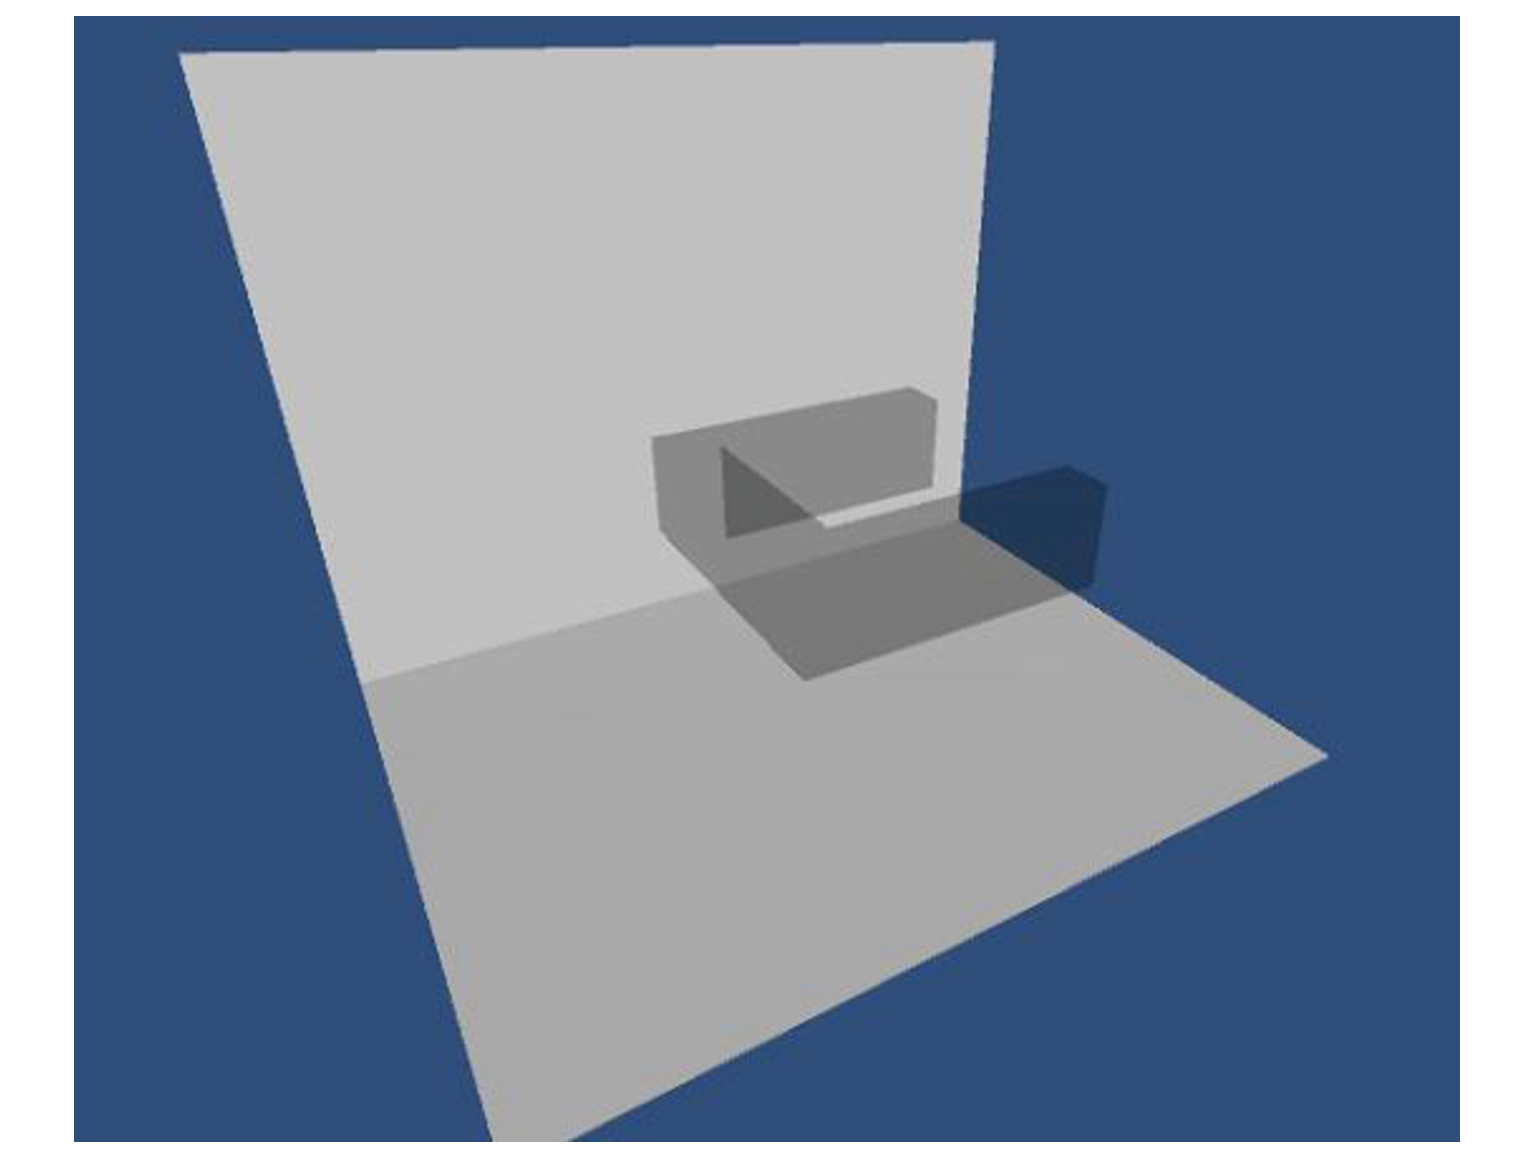
\includegraphics[width=70mm]{3d_obje_2.eps}
   図5-1. 作成した3Dオブジェクト
  \end{center}
  \label{fig:one}
 \end{minipage}
 \begin{minipage}{0.5\hsize}
  \begin{center}
   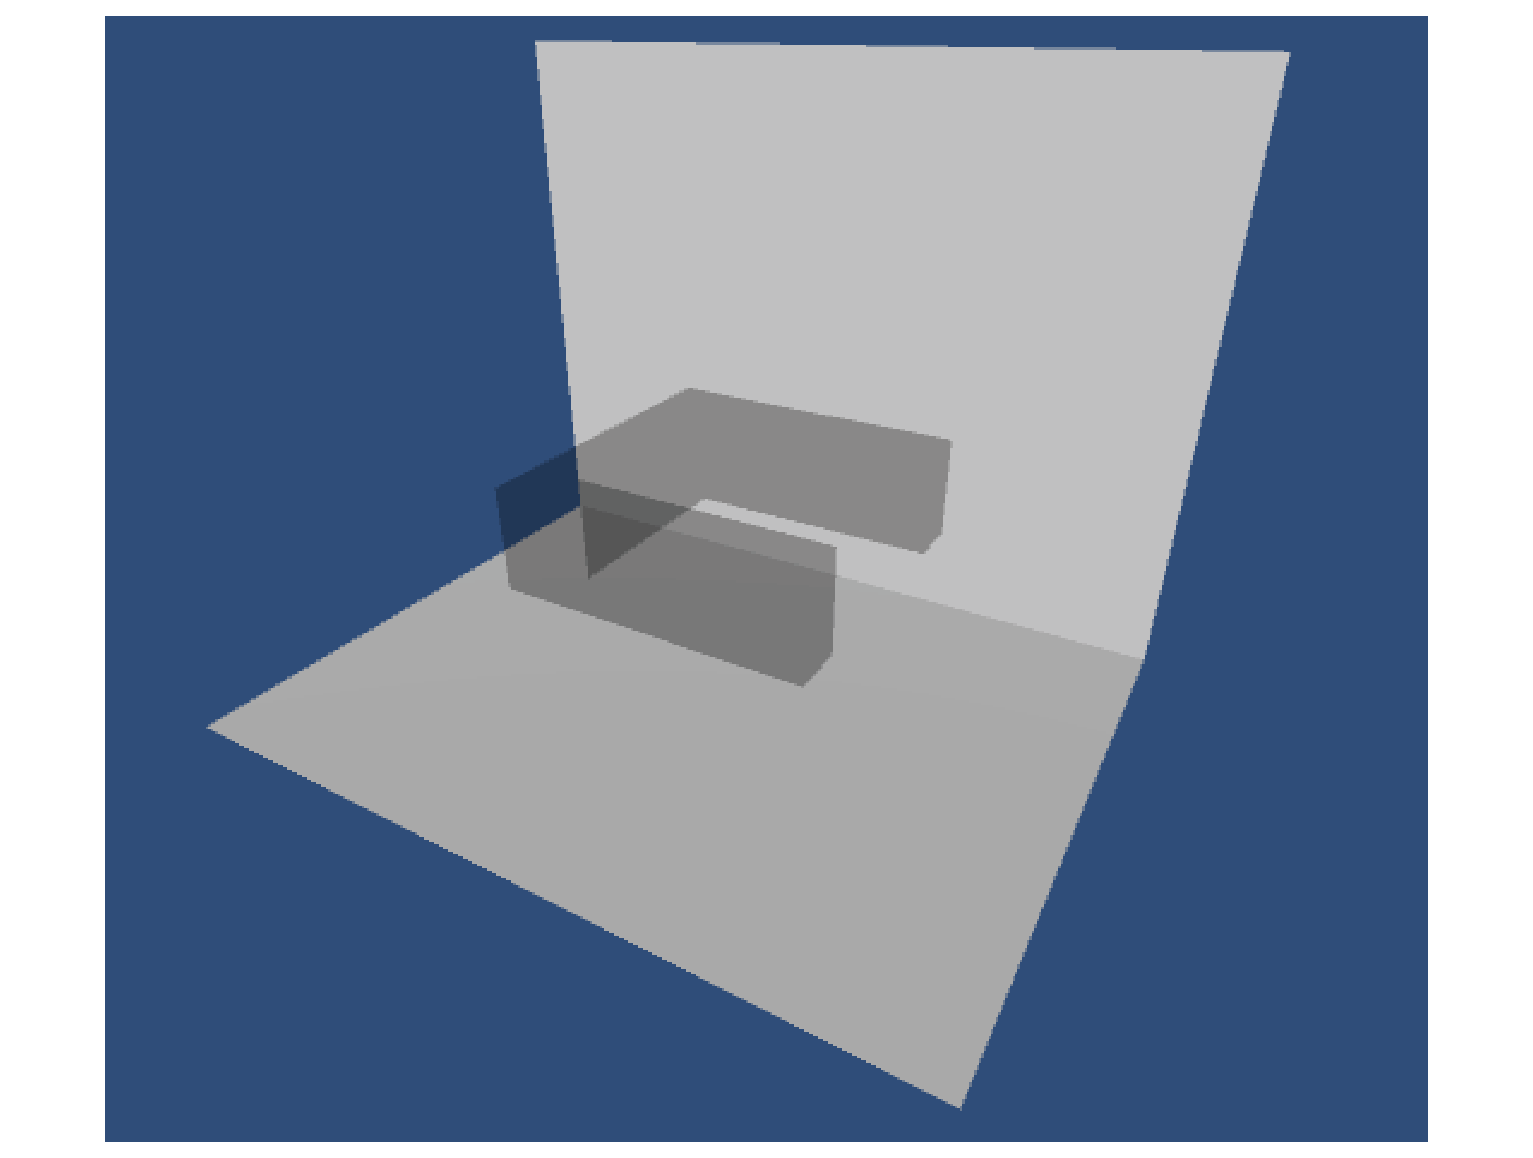
\includegraphics[width=70mm]{3d_obje_1.eps}
   図5-2. 作成した3Dオブジェクト
  \end{center}
  \label{fig:two}
 \end{minipage}

このオブジェクトに対して、3D格子点の内部外部判定を行う。結果は、図5-3となる。

 \vspace{5mm}
\begin{minipage}{0.5\hsize}
  \begin{center}
   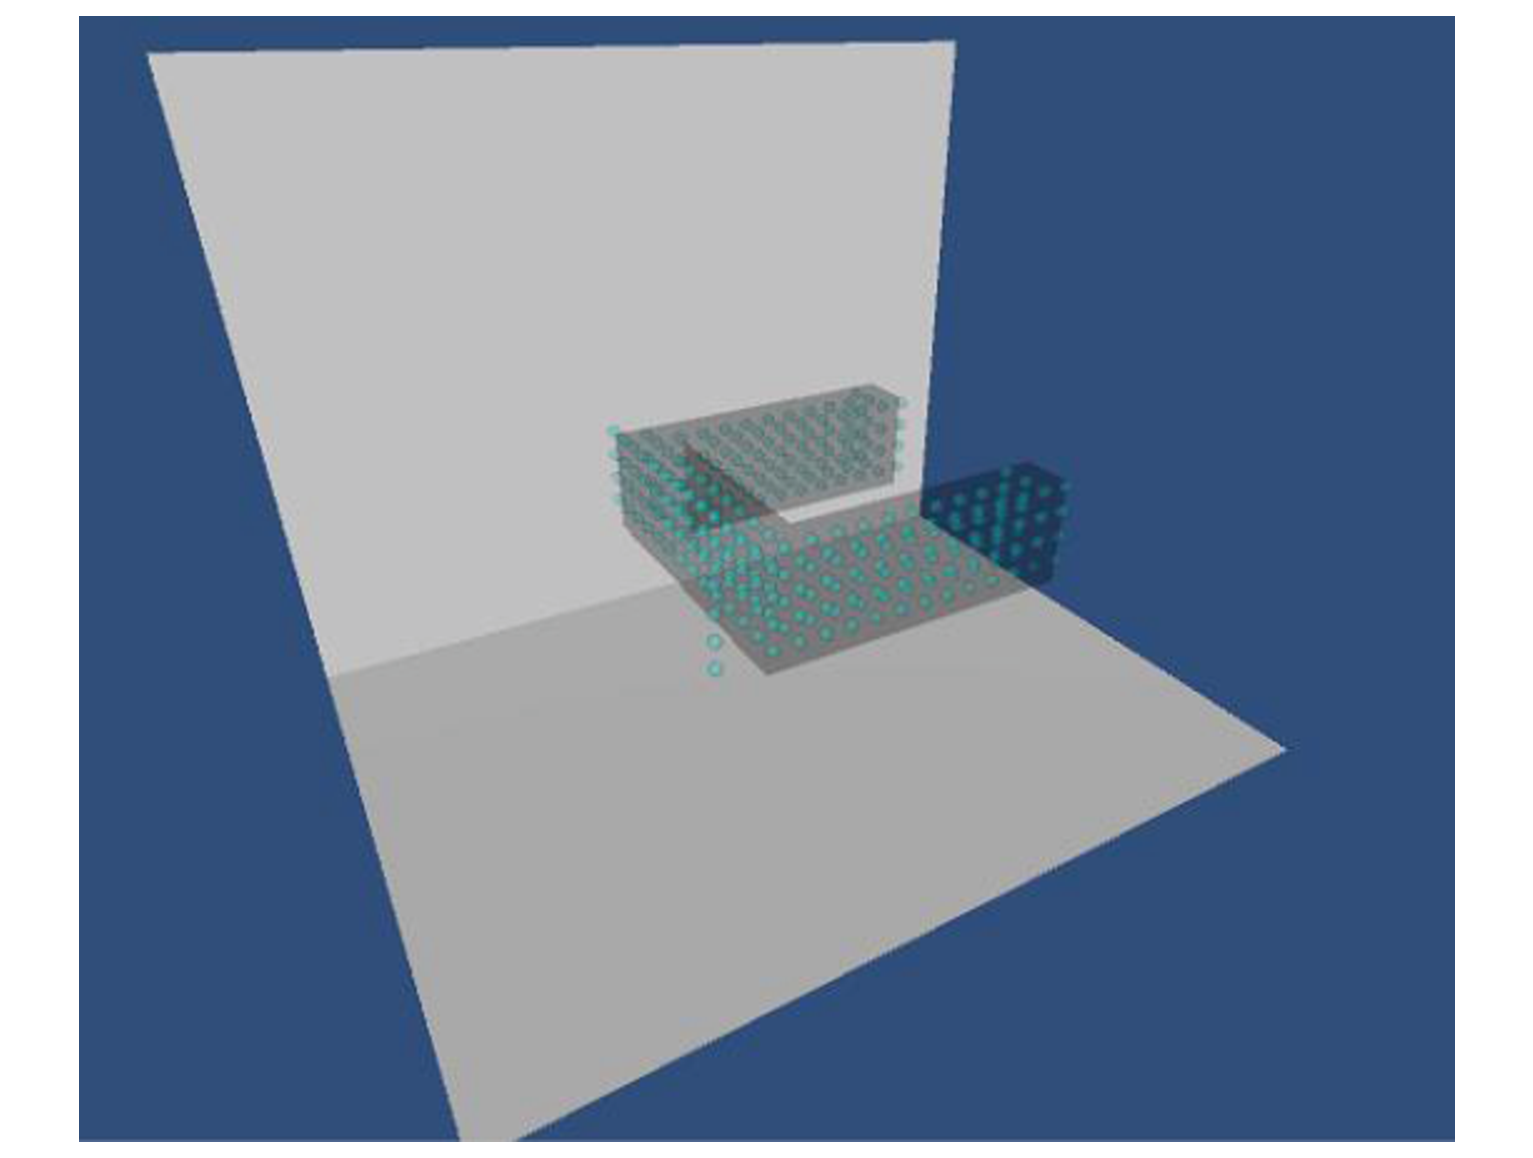
\includegraphics[width=70mm]{IED3D_2.eps}
   図5-3. 内部外部判定結果
  \end{center}
  \label{fig:one}
 \end{minipage}
 \begin{minipage}{0.5\hsize}
  \begin{center}
   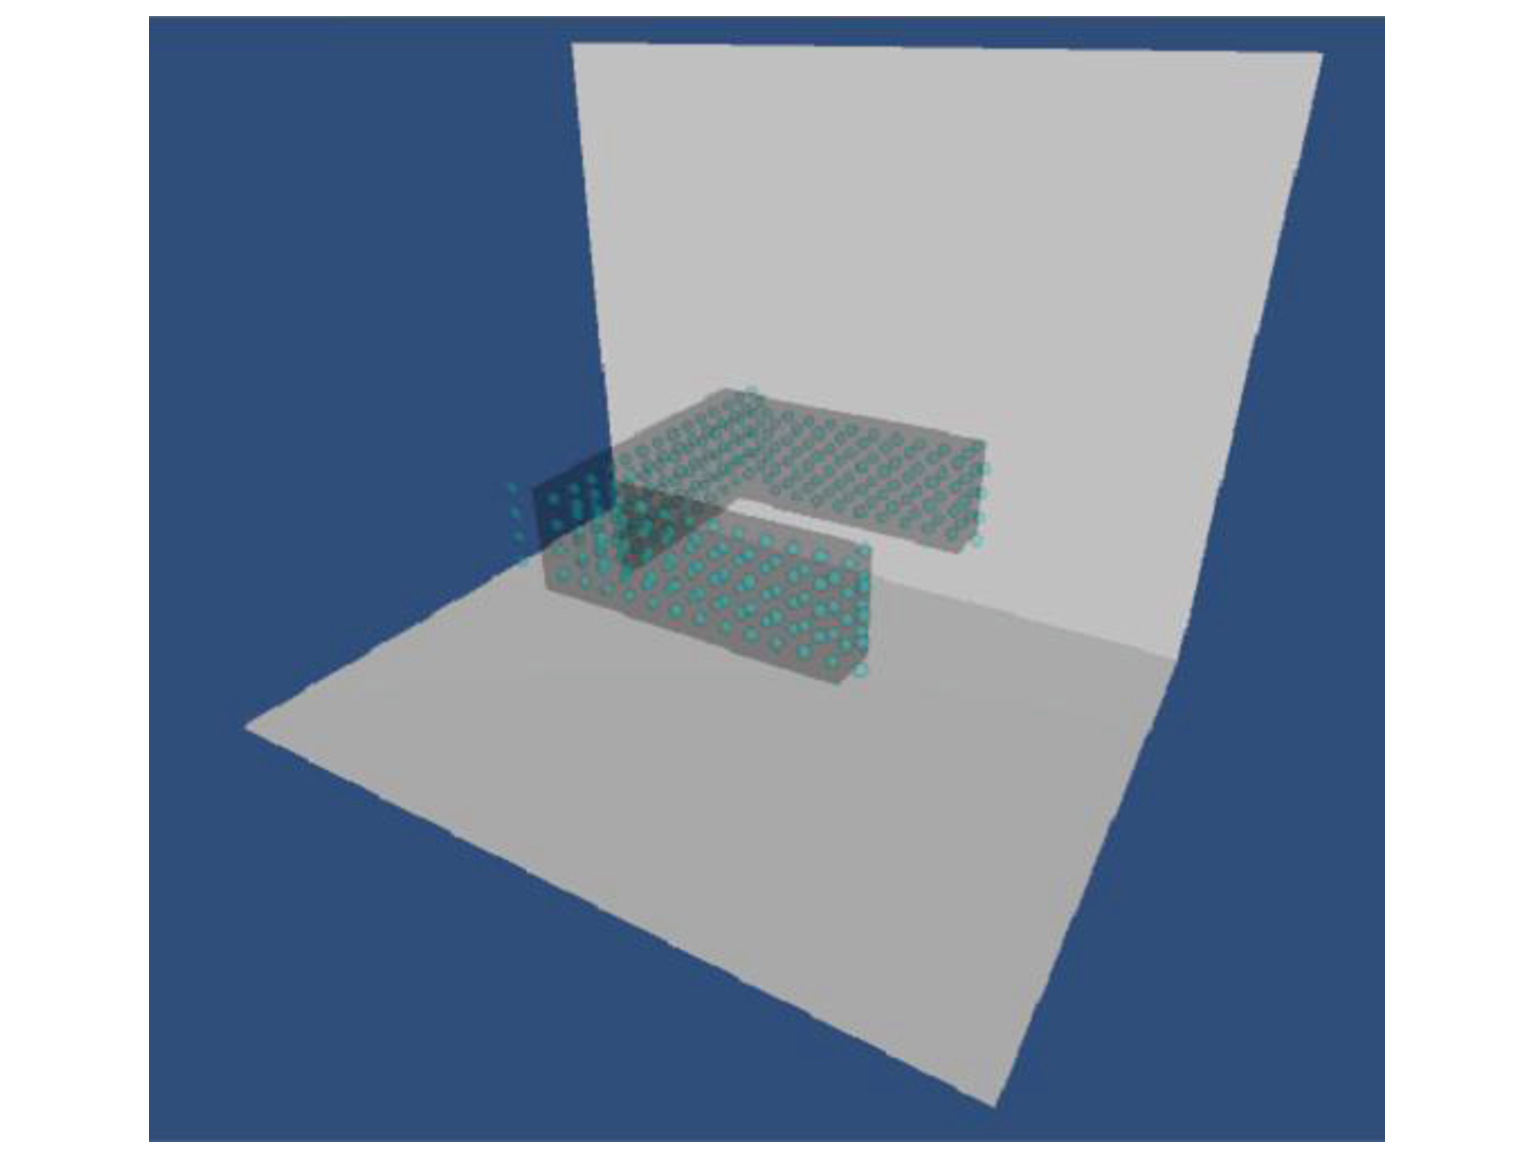
\includegraphics[width=70mm]{IED3D_1.eps}
   図5-4. 内部外部判定結果
  \end{center}
  \label{fig:two}
 \end{minipage}

青緑色の球が、内部と判定された格子点となる。若干の誤判定はあるが、概ね見た目通りに内部外部を判定できていることがわかる。ここで、3Dオブジェクトの窪んだ部分に手を挿入することで、内部外部判定を用いた当たり判定が正常に動作していることを確認する。

 \vspace{5mm}
\begin{minipage}{0.5\hsize}
  \begin{center}
   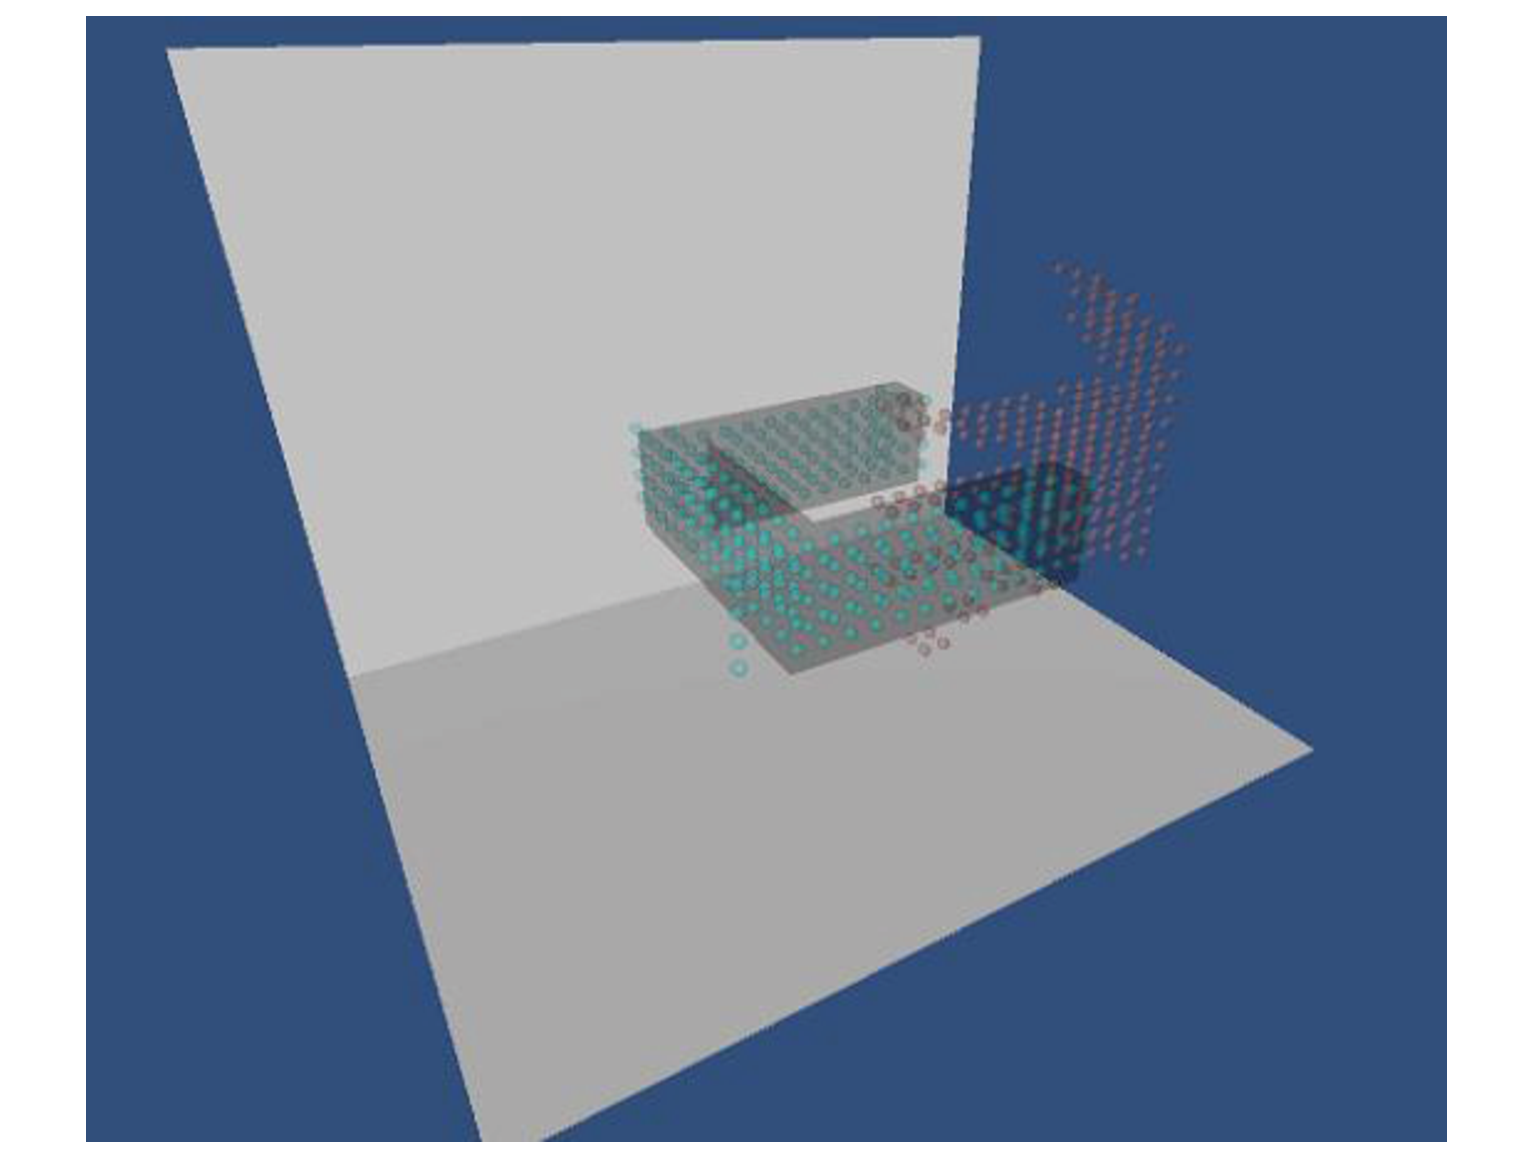
\includegraphics[width=70mm]{3D_obje_insert_1.eps}
   図5-5. 手をオブジェクトの窪みに挿入
  \end{center}
  \label{fig:one}
 \end{minipage}
 \begin{minipage}{0.5\hsize}
  \begin{center}
   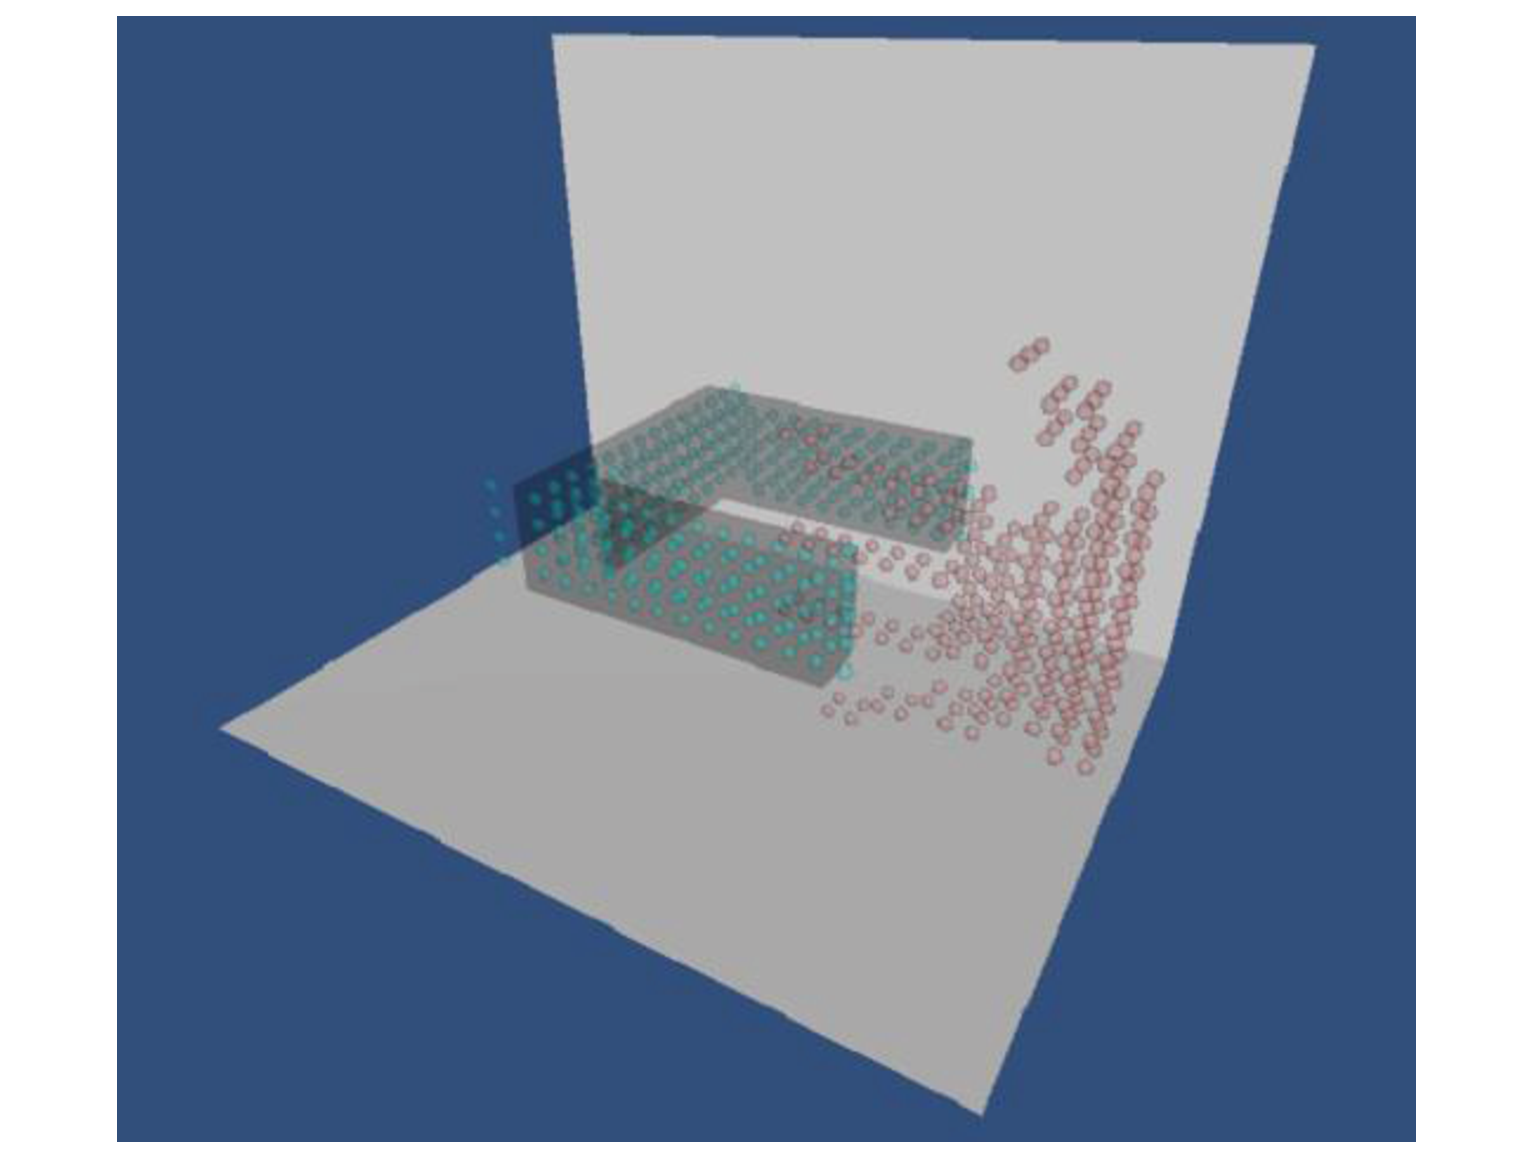
\includegraphics[width=70mm]{3D_obje_insert_2.eps}
   図5-6. 手をオブジェクトの窪みに挿入
  \end{center}
  \label{fig:two}
 \end{minipage}
 
 図5-5、図5-6の赤い点で描写されているものが、手と認識された情報を可視化したものである。窪んだ部分に手を挿入しても、3Dオブジェクトが移動しないことが確認できた。この状態で、手前に動かした結果を図5-7、図5-8に示す。
 
  \vspace{5mm}
\begin{minipage}{0.5\hsize}
  \begin{center}
   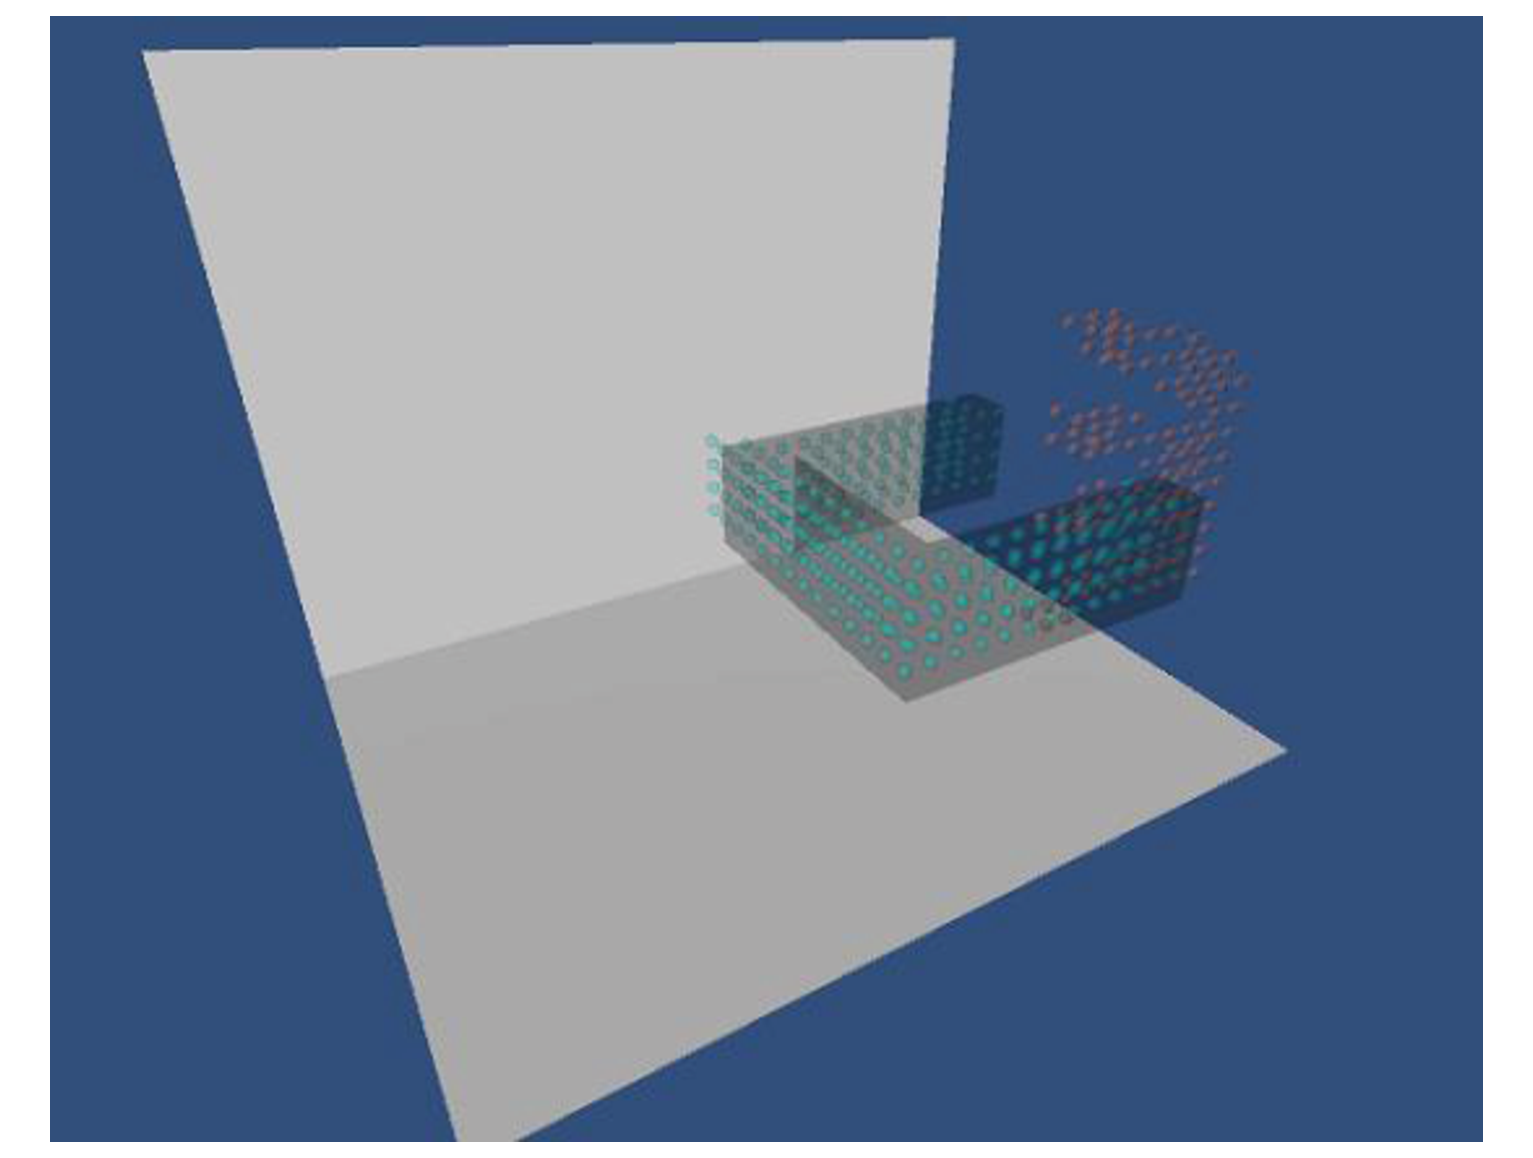
\includegraphics[width=70mm]{temae_1.eps}
   図5-5. 手を手前に移動
  \end{center}
  \label{fig:one}
 \end{minipage}
 \begin{minipage}{0.5\hsize}
  \begin{center}
   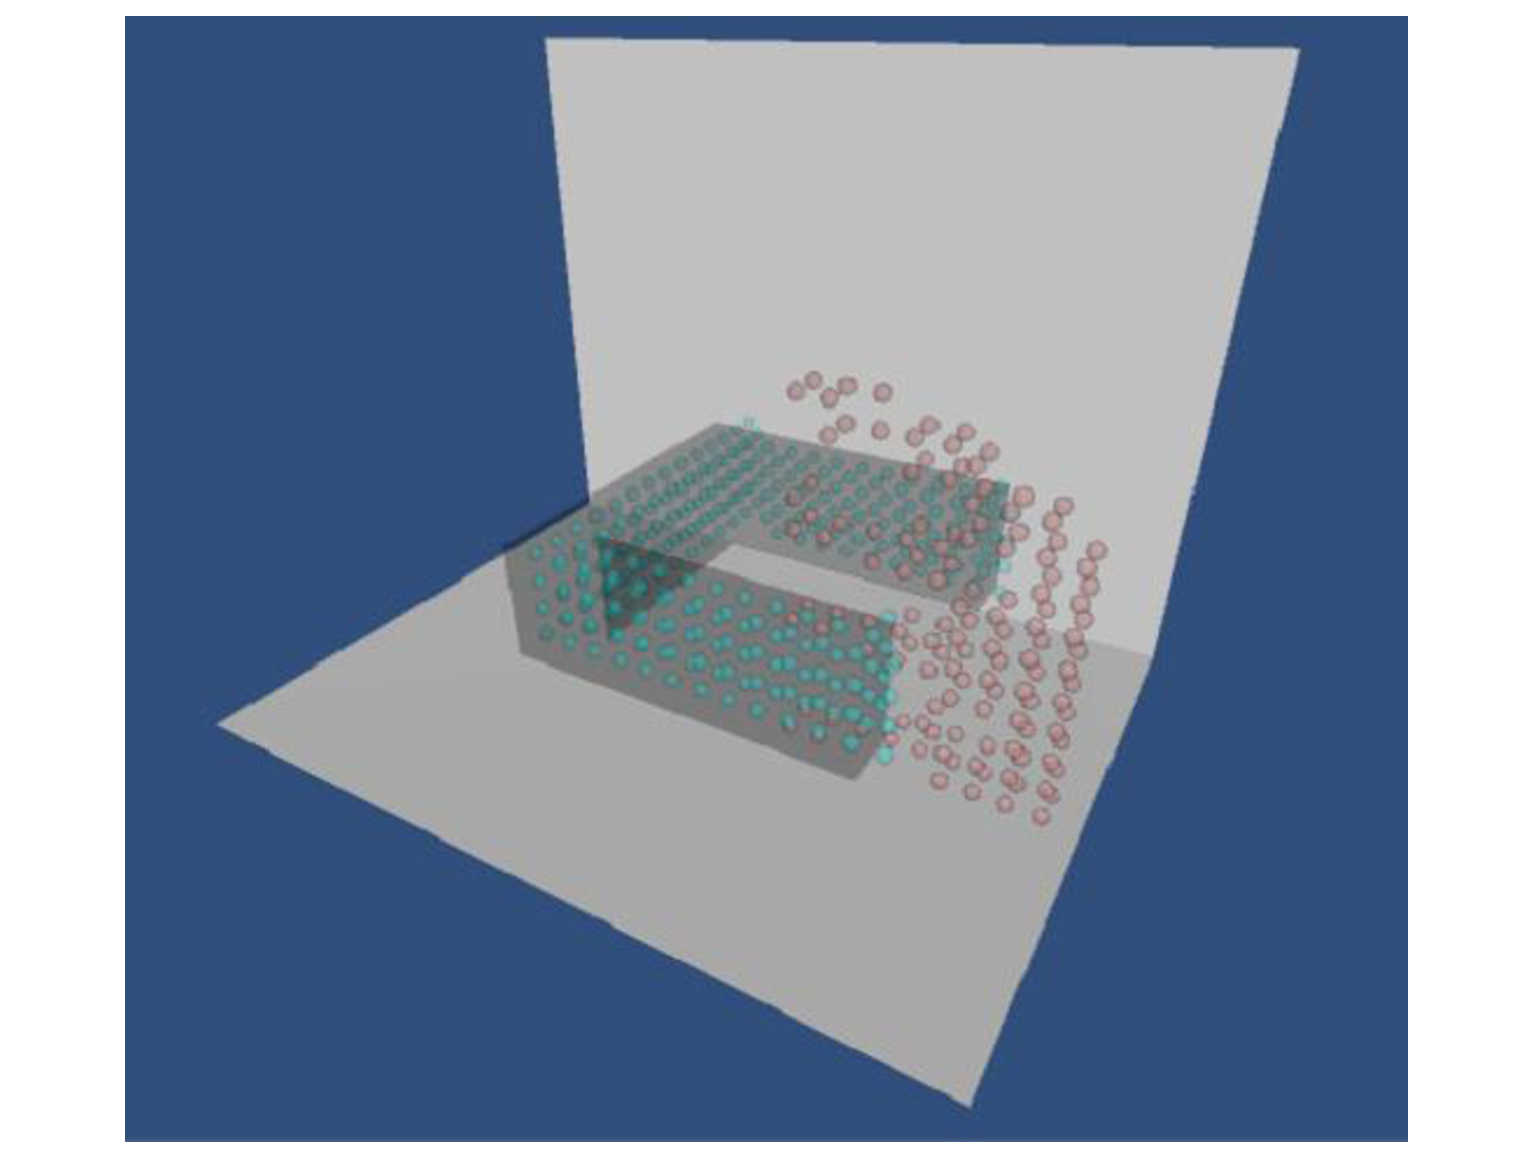
\includegraphics[width=70mm]{temae_2.eps}
   図5-6. 手を手前に移動
     \end{center}
  \label{fig:two}
 \end{minipage}
 
 手がオブジェクトに触れるのと連動して、3Dオブジェクトも手前に移動することが確認できた。これらの結果から、内部外部判定を用いた接触判定は正常に動作していることが確認できる。
 
 
 	% 実験
\newpage
% 7
\section{総括}

% 7.1
\subsection{システムについて}
本研究での目的を改めて述べる。一つは、ハンドジェスチャーとVR技術を組み合わせることによって、直感的な操作を行うことができるインターフェースの作成である。二つ目は、カメラを使用しないことにより、これまで利用できなかったシチュエーションでもジェスチャーを利用可能にする、ということである。

二つ目の、カメラを使用しないジェスチャーの利用についてだが、十分に要件を満たしていると考えている。今回使用したシミュレータデバイスだが、実際の光レーザーを使用したデバイスのデータと、ほぼ同じ形でデータを取得することができる。すなわち、4章の図4-3の格子点と同じ数だけのレーザー、および受光器を用意することができれば、Webカメラによるシミュレータでなくとも、今回の実験と同様の結果が得られることが推察できる。しかしながら、必要となるレーザー光を計算すると、縦、横それぞれにおいて、$32 \times 24$ 個を使用することになり、合計で1536個のレーザー光を使用することになる。これを一個人で用意することは難しいため、実際にデバイスを作成しようとすると、一企業単位の組織が必要となる。

一つ目の直観的な操作ができるインターフェースについてだが、今回実現できたとは言うことはできない。その原因だが、内部外部判定を行う際の、計算速度が問題としてあげられる。本システムでは、オブジェクトと手が重なった際に、オブジェクトを移動させて、再度内部外部判定を行っている。この内部外部判定の計算に時間がかかるため、あまりにも早く手を動かすと、計算が追い付かなくなり手がオブジェクトに食い込んでしまう。これにより、オブジェクトの挙動が想定外のものとなってしまう。これを解決するためには、より早い内部外部判定アルゴリズムを導入する必要があると考えられる。

% 7.2
\subsection{実験結果について}
概ね想定通りの結果を示したが、第6章の図6-3、6-4での内部外部の誤判定は想定外のものとなった。同様のアルゴリズムを用いた、第4章の図4-13では、実験で使用した図形より複雑なものにも関わらず、内部外部の誤判定は起こらなかったからである。この誤判定は図形の境界線付近で起こっているため、改良型の外積計算によって生じている。おそらく、入力される図形が第4章の図5-13のようにある程度複雑な図形の場合は、このような誤判定は起こらないが、今回の実験のように、あまりにもシンプルすぎる図形の場合、誤判定が起こるのと予想される。本研究の最終目標はVR技術との組み合わせで、インターフェースを作ることである。従って、三点のみで構成されている、あまりにもシンプルすぎる図形を想定していない。ある程度複雑な図形を想定しているため、全て第4章、4.3.3 の計算を適用している。そのことが、今回の誤判定につながったと考えられる。


% 7.3
\subsection{発展}
三次元オブジェクトの内部外部判定を行う際に、層毎に分けることで二次元の内部外部判定を行っている。この手法でも、十分な判定結果を得られるが、三次元を三次元のまま考えて内部外部判定を行う手法を用いると、同様かそれ以上の結果を得られると考えられる。従って、より正確な結果を得るためにも、今後はそのような手法について模索するべきだと考えられる。しかしながら、計算量が大幅に増えることは確実であり、これを解決するための手段も同時に考えなければならない。
	% 総括
\newpage
%%% 8
\section{謝辞}
感謝	% 謝辞
%%\newpage

% 参考文献
%参考文献
\begin{thebibliography}{9}

\bibitem{タグ1}
非凸形状を有する平面図形の形状認識に関するベクトル解析的手法の問題点., 数理解析研究所講究録 第 1544 巻 2007 年 8-12
\bibitem{タグ2}
児玉賢史, 複雑形状認識の問題点と対処方法, 数理解析研究所講究録, 第 1643 巻 2009 年 148-156
\bibitem{タグ3}
Inclusion of a Point in a Polygon - Geometry Algorithms,
http://geomalgorithms.com/a03-\_inclusion.html

\end{thebibliography} 
%\newpage

% 付録
%\input{./appendix.tex}
%\newpage

\end{document}


